\documentclass[tikz,border=10pt]{standalone}

\usetikzlibrary{lindenmayersystems}

\begin{document}

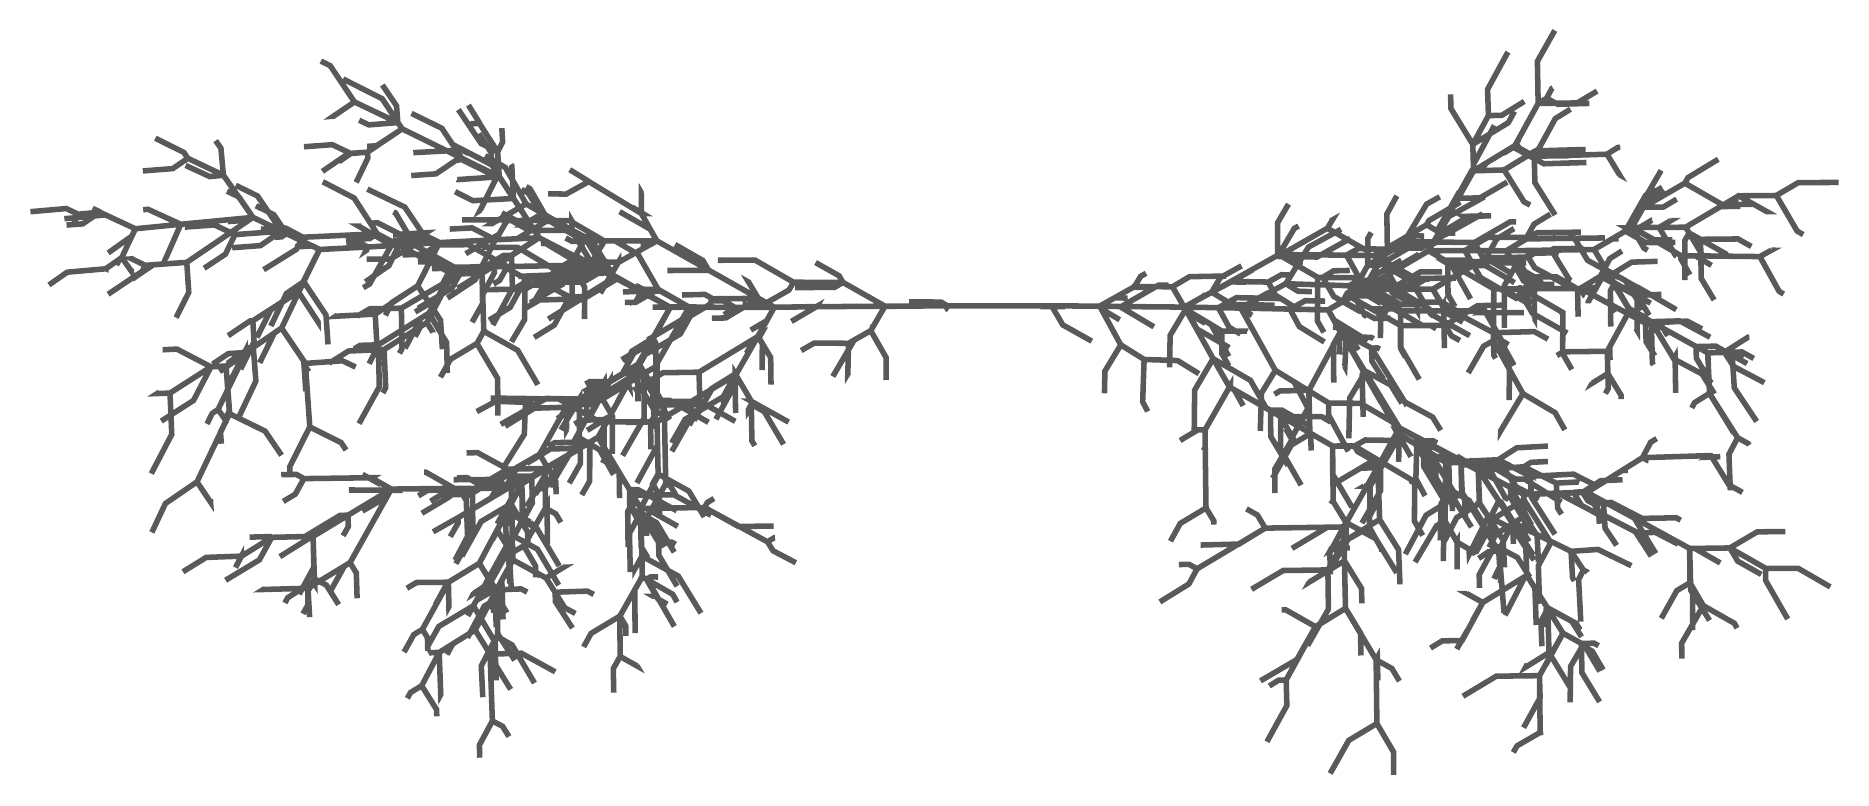
\begin{tikzpicture}[scale=5]
  
  % Single mirrored tree pair - different parameters for variation
  \pgfmathsetmacro{\treeorder}{4}
  \pgfmathsetmacro{\treestep}{1.5}
  \pgfmathsetmacro{\treeangle}{30}
  \pgfmathsetmacro{\treecolor}{70}
  
  % Left-growing fractal (mirrored)
  \begin{scope}[xscale=-1, shift={(-0.4cm, 0cm)}]
    \draw[gray!\treecolor!black, line width=2pt,
      l-system={
        rule set={F -> FF-[-F+F]+[+F-F]},
        axiom=F,
        order=\treeorder,
        step=\treestep pt,
        randomize step percent=35,
        angle=\treeangle,
        randomize angle percent=10
      }]
      lindenmayer system;
  \end{scope}
  
  % Right-growing fractal
  \begin{scope}[shift={(0.4cm, 0cm)}]
    \draw[gray!\treecolor!black, line width=2pt,
      l-system={
        rule set={F -> FF-[-F+F]+[+F-F]},
        axiom=F,
        order=\treeorder,
        step=\treestep pt,
        randomize step percent=35,
        angle=\treeangle,
        randomize angle percent=10
      }]
      lindenmayer system;
  \end{scope}
  
\end{tikzpicture}

\end{document}

